\documentclass[12pt]{article}
\usepackage{fullpage}

\usepackage[T1]{fontenc}
\usepackage[utf8]{inputenc}
\usepackage{lmodern}
\usepackage{microtype}
\usepackage[full]{textcomp}
\usepackage[osf]{newtxtext}
\usepackage{graphicx}

%% ---- Base math packages (always available) -------------------------------
\usepackage{amsmath, amssymb, amsthm, mathtools}
\usepackage{hyperref}

%% ---- Submission preamble (imported so the inlined solution compiles) ----
\usepackage{amsmath,amssymb,amsthm,mathtools}

\newtheorem{theorem}{Theorem}
\newtheorem{lemma}[theorem]{Lemma}
\newtheorem{definition}[theorem]{Definition}
\newtheorem{remark}[theorem]{Remark}

\DeclareMathOperator{\Hilb}{Hilb}
\DeclareMathOperator{\Inv}{inv}
\DeclareMathOperator{\OP}{OP}
\DeclareMathOperator{\Sym}{Sym}

\newcommand{\C}{\mathbb{C}}
\newcommand{\Sn}{\mathfrak{S}_n}
\newcommand{\qint}[1]{[#1]_q}

%% ---- Theorem environments not supplied by the submission ------------------
\makeatletter
\@ifundefined{theorem}{\newtheorem{theorem}{Theorem}}{}
\@ifundefined{lemma}{\newtheorem{lemma}{Lemma}}{}
\@ifundefined{proposition}{\newtheorem{proposition}{Proposition}}{}
\@ifundefined{corollary}{\newtheorem{corollary}{Corollary}}{}
\@ifundefined{definition}{\theoremstyle{definition}\newtheorem{definition}{Definition}}{}
\@ifundefined{remark}{\theoremstyle{remark}\newtheorem{remark}{Remark}}{}
\makeatother

%% ---- First Proof theme + in-text comment box -----------------------------
%% Palette from the FINAL DELIVERABLES brand assets:
%%   slate     #171313  (ink)
%%   warm-gray #69626D  (secondary)
%%   sand      #F2ECE9  (light background)
\usepackage{xcolor}
\usepackage[most]{tcolorbox}

\definecolor{FPslate}{HTML}{171313}
\definecolor{FPwarmgray}{HTML}{69626D}
\definecolor{FPsand}{HTML}{F2ECE9}

% Reviewer number for this document (set per file). Used by the comment box tag.
\newcommand{\reviewernum}{1}

% \review{...} : a First-Proof-themed reviewer comment, set inline in the text
%            as a sand box with a warm-gray rule and a "Reviewer N" tag.
\newtcolorbox{reviewbox}{
  breakable, enhanced, sharp corners,
  colback=FPsand, colframe=FPwarmgray,
  coltext=FPslate, boxrule=0pt, leftrule=2.5pt,
  left=8pt, right=8pt, top=14pt, bottom=5pt,
  before skip=6pt, after skip=6pt,
  fontupper=\small,
  overlay unbroken and first={
    \node[anchor=north east, font=\bfseries\footnotesize\sffamily,
          text=FPwarmgray, inner sep=0pt]
      at ([xshift=-8pt,yshift=-4pt]frame.north east) {Reviewer~\reviewernum};}
}
\newcommand{\review}[1]{\begin{reviewbox}#1\end{reviewbox}}

\title{Review of Submission 9C}
\author{First Proof Second Batch \\ Reviewer \reviewernum}
\date{June 4--8, 2026}

\makeatletter
\renewcommand{\maketitle}{%
  \noindent
  \begin{minipage}[t]{0.68\textwidth}
    \vspace{20pt}
    \raggedright
    {\LARGE\bfseries \@title\par}
    \vspace{0.35em}
    {\large \@author\par}
    \vspace{0.35em}
    {\normalsize \@date\par}
  \end{minipage}%
  \hfill
  \begin{minipage}[t]{0.25\textwidth}
    \vspace{0pt}
    \raggedleft
    \raisebox{\dimexpr-\height+\ht\strutbox+0.225in\relax}{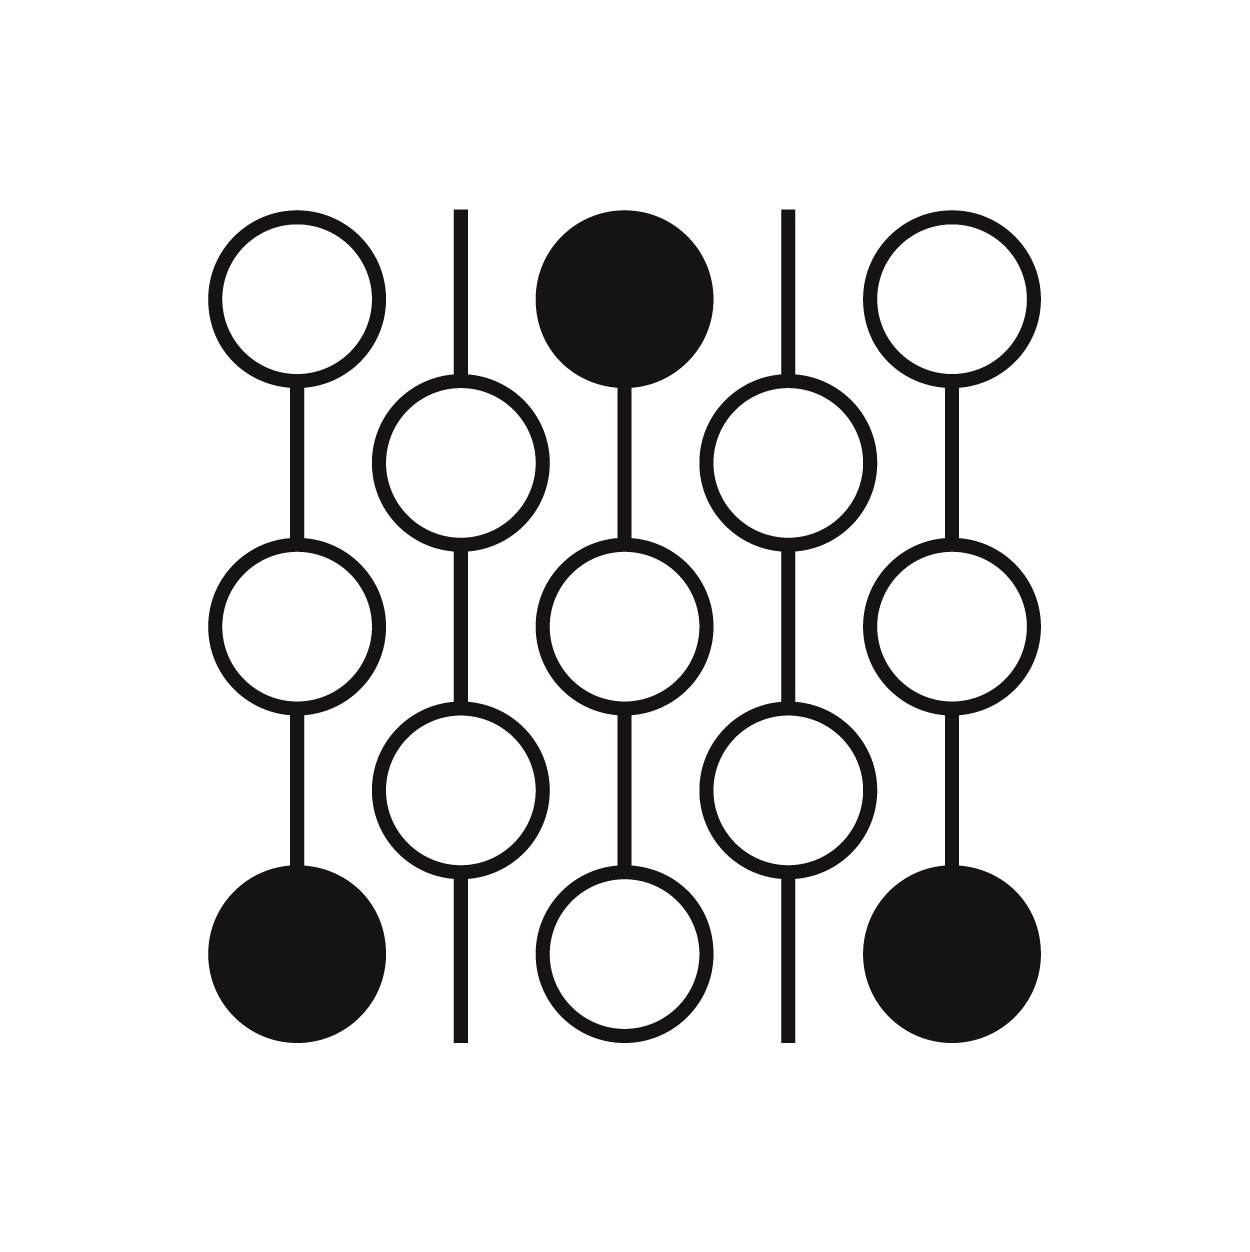
\includegraphics[height=1.35in]{Logo-slate.png}}
  \end{minipage}
  \par\vspace{2em}
}
\makeatother

\begin{document}
\maketitle
\section{Review}
The proposed solution gives a combinatorial formula for the coefficients $c_\lambda(n)$ in terms of triples $(r,\pi,t)$, where $r$ and $t$
are integers and $\pi$ is an ordered set partition.


The proof relies on Rhoades–Wilson's formula \cite{RhoadesWilson} for the Hilbert series of the super coinvariant ring $SR_n$ in terms of $q$-Stirling numbers. Using classical combinatorial results on Stirling numbers, together with elementary manipulations of $q$-identities, this Hilbert series is then rewritten as a generating function of decorated integer partitions.

Here are some comments:
\begin{itemize}
    \item An important step in the argument is to use the universality of the coefficients $c_\lambda(n)$ which allows one to extract them from the Hilbert series of $SR_n$. This step does not seem to be explained clearly enough (see also the related comments on Lemma 3).
    \item Some references are missing, others are not sufficiently accurate.
\end{itemize}

\paragraph{Correctness.}
The combinatorial formula is correct, as are the main steps of the proof.

\paragraph{Novelty.}
The proof starts by relating the coefficients in question to the Hilbert series of the super coinvariant ring $SR_n$ as expected, however it does not seem to cite the correct references.

The proof then uses standard references to connect this Hilbert series to the combinatorics of $q$-Stirling numbers. The trick used to factorize the series $H_n(q,z)$ (see Lemma 4) simplifies the final step of the proof. 

The combinatorial interpretation in terms of ordered set partitions is then expected, however the use of the extra integer $t$ makes the final formula feel slightly  ``less natural''.

\section{Recommendation}
The formula is correct and the solution is well written except for minor citation issues. I recommend publication after minor revisions.


  \section{Submission with inline comments}

%% ======================================================================
%% Inlined verbatim from the anonymised submission prob_009-C.
%% ======================================================================

\date{}



\begin{abstract}
Let \(R_n^{(m)}\) be the diagonal coinvariant algebra of \(\mathfrak S_n\) in
\(m\) sets of \(n\) commuting variables, and write
\[
\Hilb(R_n^{(m)};q_1,\dots,q_m)
=
\sum_{\lambda} c_\lambda(n)s_\lambda(q_1,\dots,q_m).
\]
For hook shapes \(\lambda=(a+1,1^b)\), we give a positive ordered-set-partition
interpretation of \(c_\lambda(n)\).
\end{abstract}

\subsection{Statement of the hook formula}
\review{``Hook formula'' is not a natural name here–it usually refers to a classical formula in combinatorial representation theory.}

For \(r,k\geq 1\), let \(\OP_{r,k}\) be the set of ordered set partitions
\[
\pi=(B_1\mid B_2\mid \cdots \mid B_k)
\]
of \([r]=\{1,\dots,r\}\) into \(k\) nonempty blocks. Define
\[
\Inv(\pi)
=
\#\{(i,j,x): 1\leq i<j\leq k,\ x\in B_i,\ x>\min(B_j)\}.
\]
Also write \([k]_q=1+q+\cdots+q^{k-1}\).

\begin{theorem}[Hook coefficients]
Let \(n\geq 1\). For \(a,b\geq 0\), write the hook
\[
(a\mid b):=(a+1,1^b).
\]
Then
\[
\boxed{
\sum_{a,b\geq 0} c_{(a\mid b)}(n)\,q^a z^b
=
\sum_{r=1}^{n-1}\sum_{k=1}^{r}
z^{r-k}[k]_q
\sum_{\pi\in \OP_{r,k}} q^{\Inv(\pi)}.
}
\]
Equivalently,
\[
\boxed{
c_{(a+1,1^b)}(n)
=
\#\left\{
(r,\pi,t):
\begin{array}{l}
1\leq r\leq n-1,\ \pi\in \OP_{r,r-b},\\
0\leq t\leq r-b-1,\ \Inv(\pi)+t=a
\end{array}
\right\}.
}
\]
In particular, \(c_{(a+1,1^b)}(n)=0\) unless \(0\leq b\leq n-2\).
\end{theorem}

\subsection{Ordered set partitions and \(q\)-Stirling numbers}

Let
\[
A_{r,k}(q):=\sum_{\pi\in \OP_{r,k}} q^{\Inv(\pi)}.
\]

\begin{lemma}
The polynomials \(A_{r,k}(q)\) satisfy
\[
A_{r,k}(q)=[k]_q\bigl(A_{r-1,k}(q)+A_{r-1,k-1}(q)\bigr),
\]
with \(A_{1,1}(q)=1\). Hence
\[
A_{r,k}(q)=[k]!_q\,\mathrm{Stir}_q(r,k),
\]
where \(\mathrm{Stir}_q(r,k)\) is the Carlitz \(q\)-Stirling number defined by
\[
\mathrm{Stir}_q(r,k)=[k]_q\,\mathrm{Stir}_q(r-1,k)+\mathrm{Stir}_q(r-1,k-1).
\]
\end{lemma}

\begin{proof}
Remove the largest element \(r\) from an ordered set partition
\(\pi=(B_1|\cdots|B_k)\).

If \(r\) lies in a block \(B_i\) of size at least \(2\), removing \(r\) gives an
ordered set partition in \(\OP_{r-1,k}\). Conversely, inserting \(r\) into block
\(i\) of a partition in \(\OP_{r-1,k}\) creates exactly \(k-i\) new inversions,
since \(r>\min(B_j)\) for every block \(j>i\). Thus these insertions contribute
\[
\sum_{i=1}^k q^{k-i} A_{r-1,k}(q)=[k]_q A_{r-1,k}(q).
\]

If \(r\) is a singleton block, deleting that block gives a partition in
\(\OP_{r-1,k-1}\). Conversely, inserting the singleton block \(\{r\}\) in
position \(i\) creates again \(k-i\) new inversions. These insertions contribute
\([k]_q A_{r-1,k-1}(q)\). Adding the two cases proves the recurrence. The
identification with \([k]!_q\mathrm{Stir}_q(r,k)\) follows from the same recurrence
and initial condition.
\end{proof}

\subsection{Superspace and hook extraction}

Let \(\Omega_n=\C[x_1,\dots,x_n]\otimes \bigwedge(\theta_1,\dots,\theta_n)\), where
the \(x_i\) commute and the \(\theta_i\) anticommute. Let \(\Sn\) act diagonally by
\[
w\cdot x_i=x_{w(i)},\qquad w\cdot \theta_i=\theta_{w(i)}.
\]
The superspace coinvariant ring is
\[
SR_n:=\Omega_n/\langle(\Omega_n)^{\Sn}_+\rangle.
\]
\review{I think that $(\Omega_n)_+$ has not been defined.}
Let \(q\) track \(x\)-degree and \(z\) track \(\theta\)-degree.

\begin{lemma}[Hook specialization]
Let
\[
C_n(q,z):=\sum_{a,b\geq 0} c_{(a\mid b)}(n)q^a z^b.
\]
Then
\[
\Hilb(SR_n;q,z)=1+(q+z)C_n(q,z).
\]
\end{lemma}

\begin{proof}
The construction of diagonal coinvariants is functorial in the row-space. 
\review{This sentence is ambiguous.}
For a
purely even row-space of dimension \(m\), its character is
\[
\sum_\lambda c_\lambda(n)s_\lambda(q_1,\dots,q_m).
\]
Evaluating the same polynomial functor on a \(1|1\)-dimensional superspace gives
the superspace coinvariant ring \(SR_n\). 
\review{A reference is mussing here, I think that Lentfer 2025 should be cited for this result.}
By the Berele--Regev hook Schur
character theory, the ordinary Hilbert character of the Schur functor
\(\mathbb S_\lambda\) on one even variable \(q\) and one odd variable \(z\) is zero
unless \(\lambda\) is a hook. Moreover,
\[
hs_{(a\mid b)}(q;z)=q^{a+1}z^b+q^a z^{b+1}=(q+z)q^a z^b,
\]
and \(hs_\varnothing(q;z)=1\). Therefore
\[
\Hilb(SR_n;q,z)
=
1+\sum_{a,b\geq 0}c_{(a\mid b)}(n)(q+z)q^a z^b
=
1+(q+z)C_n(q,z).
\]
\review{Give a reference for this formula.}
This is the standard hook Schur specialization; see Berele--Regev
\cite{BereleRegev} or Macdonald \cite[Ch.~I, \S3, Ex.~23]{Macdonald}.
\review{The references given are not the relevant ones here; this follows from the previous formula and the fact that the Hilbert series and the observation above on superspace coinvariant ring $SR_n$.}
\end{proof}

\subsection{Hilbert series of \(SR_n\)}

Rhoades and Wilson proved the following Hilbert series formula for the superspace
coinvariant ring \cite[Theorem~1.1 and Eq.~(1.10)]{RhoadesWilson}:
\review{Only Eq. (1.10) should be cited, Theorem 1.1 does not exist in \cite{RhoadesWilson}.}
\[
\Hilb(SR_n;q,z)=
\sum_{k=1}^{n} z^{n-k}[k]!_q\,\mathrm{Stir}_q(n,k).
\]
Using the preceding lemma, this can be written as
\[
\Hilb(SR_n;q,z)=
\sum_{k=1}^{n}z^{n-k}A_{n,k}(q).
\]

Set
\[
H_n(q,z):=\sum_{k=1}^{n}z^{n-k}A_{n,k}(q).
\]
Then \(H_1(q,z)=1\).

\begin{lemma}
For \(n\geq 2\),
\[
H_n(q,z)-H_{n-1}(q,z)
=
(q+z)\sum_{k=1}^{n-1} z^{n-1-k}[k]_q A_{n-1,k}(q).
\]
Consequently,
\[
\frac{H_n(q,z)-1}{q+z}
=
\sum_{r=1}^{n-1}\sum_{k=1}^{r}
z^{r-k}[k]_q A_{r,k}(q).
\]
\end{lemma}

\begin{proof}
Using the recurrence from the ordered-set-partition lemma,
\[
A_{n,k}=[k]_q(A_{n-1,k}+A_{n-1,k-1}).
\]
Therefore
\[
\begin{aligned}
H_n
&=
\sum_{k=1}^{n} z^{n-k}[k]_qA_{n-1,k}
+
\sum_{k=1}^{n} z^{n-k}[k]_qA_{n-1,k-1}  \\
&=
\sum_{k=1}^{n-1} z^{n-k}[k]_qA_{n-1,k}
+
\sum_{k=1}^{n-1} z^{n-1-k}[k+1]_qA_{n-1,k} \\
&=
\sum_{k=1}^{n-1} z^{n-1-k}
\bigl(z[k]_q+[k+1]_q\bigr)A_{n-1,k}.
\end{aligned}
\]
Since
\[
z[k]_q+[k+1]_q
=
z[k]_q+1+q[k]_q
=
1+(q+z)[k]_q,
\]
we obtain
\[
H_n
=
H_{n-1}
+
(q+z)\sum_{k=1}^{n-1} z^{n-1-k}[k]_qA_{n-1,k}.
\]
Telescoping from \(H_1=1\) proves the second formula.
\end{proof}

\subsection{Proof of the theorem}

By the hook-specialization lemma and the Rhoades--Wilson Hilbert series formula,
\[
1+(q+z)C_n(q,z)
=
H_n(q,z).
\]
Thus
\[
C_n(q,z)=\frac{H_n(q,z)-1}{q+z}.
\]
The preceding lemma gives
\[
C_n(q,z)
=
\sum_{r=1}^{n-1}\sum_{k=1}^{r}
z^{r-k}[k]_qA_{r,k}(q)
=
\sum_{r=1}^{n-1}\sum_{k=1}^{r}
z^{r-k}[k]_q
\sum_{\pi\in \OP_{r,k}}q^{\Inv(\pi)}.
\]
Since
\[
[k]_q=\sum_{t=0}^{k-1}q^t,
\]
the coefficient of \(q^a z^b\) counts triples
\[
(r,\pi,t)
\]
such that \(1\leq r\leq n-1\), \(\pi\in \OP_{r,k}\), \(k=r-b\), \(0\leq t\leq k-1\),
and
\[
\Inv(\pi)+t=a.
\]
This is precisely the stated interpretation of \(c_{(a+1,1^b)}(n)\).

\begin{thebibliography}{9}

\bibitem{BereleRegev}
A.~Berele and A.~Regev,
\newblock Hook Young diagrams with applications to combinatorics and to representations of Lie superalgebras,
\newblock \emph{Adv. Math.} \textbf{64} (1987), 118--175.

\bibitem{Bergeron}
F.~Bergeron,
\newblock Multivariate diagonal coinvariant spaces for complex reflection groups,
\newblock \emph{Adv. Math.} \textbf{239} (2013), 97--108.

\bibitem{Macdonald}
I.~G. Macdonald,
\newblock \emph{Symmetric Functions and Hall Polynomials},
\newblock 2nd ed., Oxford University Press, 1995.

\bibitem{RhoadesWilson}
B.~Rhoades and A.~T. Wilson,
\newblock The Hilbert series of the superspace coinvariant ring,
\newblock \emph{Forum Math. Pi} \textbf{12} (2024), Paper No. e16.

\end{thebibliography}

\end{document}
